\section{Example}
\label{sec:example}

\begin{figure}[t]
\begin{CodeOut}
\begin{alltt}
\textbf{Java code}:
1  File file = \textbf{new} File("test");
2  Boolean b = file.exists();

\textbf{Translated C\# code}:
3  FileInfo file = \textbf{new} FileInfo("test");
4  Boolean b = System.IO.File.Exist(file.FullName)||
           System.IO.Directory.Exists(file.FullName);
\end{alltt}
\end{CodeOut}\vspace*{-4ex}
\caption{\label{fig:challenge}Java code and its translated C\# code.}%\vspace*{-1ex}
\end{figure}
\begin{figure}[t]
\begin{CodeOut}\vspace*{-1ex}
\begin{alltt}
  IndexFiles.java:
5 public class IndexFiles \{
6   static final File INDEX_DIR = new File("index");
7   public static void main(String[] args) \{
      ...
8     if (INDEX_DIR.exists()) \{...\}
      ...
9       INDEX_DIR.delete();
    \}
  \}

  IndexFiles.cs:
10 class IndexFiles\{
11   internal static readonly System.IO.FileInfo INDEX_DIR
          = new System.IO.FileInfo("index");
12   public static void  Main(System.String[] args)\{
      ...
13     bool tmpBool;
14     if (System.IO.File.Exists(INDEX_DIR.FullName))
15       tmpBool = true;
16    else
17       tmpBool = System.IO.Directory
                         .Exists(INDEX_DIR.FullName);
      ...
    \}
 \}
\end{alltt}
\end{CodeOut}\vspace*{-4ex}
\caption{\label{fig:clientcode} Two versions (Java and C\#) of
client code.}\vspace*{-2ex}
\end{figure}

We next use an example to illustrate challenges in mining 
API mapping relations. Figure~\ref{fig:challenge} shows a
Java code example and its translated C\# code. This Java code
example accepts a \CodeIn{string} input that represents the name of a
file or directory and returns a \CodeIn{boolean} value that
describes whether the file or directory exists. To achieve this functionality, the
code example declares a local variable, called \CodeIn{file}, of
type \CodeIn{java.io.File} and invokes the \CodeIn{exists} method. The
method takes the \CodeIn{string} input and \CodeIn{file} as its
inputs and produces the desirable \CodeIn{boolean} value. Here, we
consider \CodeIn{file} (a receiver) as a special input for
the \CodeIn{exists} method.

To translate this code example into C\#, a translation tool needs to
know mapping relations of API classes, so it can translate inputs,
outputs, and variables into C\#. For example, the translation tool
needs to know the mapped API class for \CodeIn{java.io.File} in C\#
to translate the variable \CodeIn{file} to C\#. In addition, the
translation tool needs to know the mapped API methods, so it can
add code for invoking proper API methods that use translated inputs and variables to
produce desirable outputs. For this example, the translation tool
adds code for invoking the \CodeIn{Exists} method and the 
\CodeIn{FullName} method to achieve the functionality. 
Here, we consider field accesses as special type of method calls.

Some projects such as Lucene have both Java and C\# versions. Our
approach has three major steps to mine the preceding two types of
mapping relations of APIs from these projects.

\textbf{Aligning client code.} First, our approach aligns classes
and methods (between the two versions) that implement similar functionality.
As these aligned classes and methods implement similar functionality,
our approach mines mapping relations of API classes and methods from
these aligned classes and methods. To align classes and methods, our approach uses a 
mapping algorithm based on similarities in the names of classes and methods. 

Aligning client code based on names of classes and methods
is based on our observation on how many existing projects such as
rasp\footnote{\url{http://sourceforge.net/projects/r-asp/}} are
migrated from one language to another. We observed that while
migrating the rasp project from C\# to Java, programmers first renamed
source files from C\# to Java and systematically addressed the
compilation errors by replacing C\# APIs with Java APIs. During this
procedure, names of classes, methods, fields of classes, or local
variables in methods often remain the same or similar between the two versions.
Therefore, we use name similarities for aligning client code of the
two versions. For example, our approach aligns
\CodeIn{IndexFiles.java} with the \CodeIn{IndexFiles.cs} (shown in
Figure~\ref{fig:clientcode}) since the names of their classes and
methods are similar.
%\begin{figure}[t]
%\centering
%\includegraphics[scale=0.65,clip]{figure/dataflow.eps}\vspace*{-3ex}
% \caption
%{\label{fig:dataflow}API methods connected by inputs and
%outputs}\vspace*{-3ex}
%\end{figure}

\textbf{Mining API mapping of classes.} Next, our approach
mines mapping relations of API classes by comparing entities such as
names of fields in aligned classes, or variable names or constants
in aligned methods. Our approach uses a text-based similarity
metric for comparing these entities and considers the entities as
similar if the metric is greater than a given threshold. These
mapping relations of API classes help translate variables from one
language to another. For example, our approach identifies the
constant value ``\CodeIn{index}'' in Lines 6 (Java) and 11 (C\#)
(Figure~\ref{fig:clientcode}) and maps the API classes associated
with these constants. Based on this constant value, our approach maps
the API class \CodeIn{java.io.File} of Java to \CodeIn{System.IO.FileInfo} of C\#.

\textbf{Mining API mapping of methods.} After mapping API classes
between the two languages, our approach maps API methods. Mapping
API methods is challenging since often an API method of one language
can be mapped to multiple API methods of the other language.
Furthermore, mapping relations of API methods should also describe
how parameters and returns are mapped between them. To address
these challenges, our approach constructs a graph, referred to as
\emph{API Transformation Graph} (ATG), for each aligned method of the
client code in both languages. These ATGs precisely capture inputs
and outputs of API methods, and help mine mapping relations of API
methods. Figure~\ref{fig:example} shows a mapping relation between
API method \CodeIn{Exists} from one language to another. (@Hao, could you please
add notations used in the figure here.)
Section~\ref{sec:approach:mappingtypes} presents more details on how
we mine these mapping relations of API methods using ATGs.
Our approach uses these mapping relations to assist translation tools such
as Java2CSharp for conducting language translation.

\begin{figure}[t]
\centering %\hfill
\includegraphics[scale=0.95,clip]{figure/sample.eps}\vspace*{-3ex}
 \caption{\label{fig:example}API mapping}\vspace*{-3ex}
\end{figure}

%Based on the mapping relations, a translation tool can migrate the
%preceding code snippet automatically. To learn the mapping
%relations,
%
%%\begin{figure}[t]
%%\centering
%%\includegraphics[scale=0.86,clip]{figure/openfile.eps}\vspace*{-1.5ex}
%% \caption
%%{\label{fig:openfile}Aligned client code}\vspace*{-2ex}
%%\end{figure}
%
%In this section, we illustrate the main steps of our approach to
%mine the API mapping in Java for \CodeIn{System.IO.Directory.
%Exists()} in C\# from the HypoLog
%project\footnote{\url{http://sourceforge.net/projects/twlog/}}.
%
%The first step of our approach is to align classes and methods of
%client code by names. This step finds class pairs and method pairs
%that implement similar functionalities, and each pair may use
%API mapping since it implements a similar functionality. Our
%approach chooses names to align classes and methods because these
%classes and methods are from the same project. In this example, our
%approach aligns the two methods as shown in
%Figure~\ref{fig:openfile} because the two method have similar names
%and their declaring classes also have similar names (see
%Section~\ref{sec:approach:alignclientcode} for details).
%
%The second step of our approach is to mine mapping relations of API
%classes based on the names of corresponding fields, parameters,
%returned types, and local variables. This step also relies on names
%for the same consideration of the first step. For example, our
%approach maps the two parameters with the same name as shown by the
%red arrow of Figure~\ref{fig:openfile}. From the types of the two
%parameters, our approach mines the mapping relation between two API
%classes: \CodeIn{System.String} $\leftrightarrow$
%\CodeIn{java.lang.String} (see
%Section~\ref{sec:approach:mappingtypes} for details).
%
%
%The final step of our approach is to mine mapping relations of API
%methods. Besides the factors listed in
%Section~\ref{sec:introduction}, another factor is that API calls in
%client code are often not carefully aligned. To deal with those
%challenges, our approach first builds an API Transformation Graph
%(ATG) for each method. After that, our approach compares built
%graphs to mine mapping relations of API methods (see
%Section~\ref{sec:approach:mappingtypes} and
%Figure~\ref{fig:approach1} for details). Figure~\ref{fig:example}
%shows the mined mapping relation between
%\CodeIn{System.IO.Directory.Exists()} and its API mapping in
%Java.
